\section{Panel operatorski}
\indent

W~poniższym rozdziale opisane zostały prace związane z~tworzeniem panelu
operatorskiego z~wykorzystaniem biblioteki \textit{Qt} w~języku \textit{C++}.
Przedstawione zostały zarówno działania zmierzające do uzyskania funkcjonalności
odpowiadającej programom typu SCADA, jak i~pewne szczegóły implementacyjne.
Również w~tym rozdziale znajduje się część porównań do programu \textit{zenon},
który stanowił w~pewnym uproszczeniu wzór do prac.

\subsection{Tworzenie oprogramowania}
\indent

Jak już zostało wspomniane, oprogramowanie zostało stworzone z~wykorzystaniem
biblioteki \textit{Qt} oraz języka \textit{C++}. Jako środowisko programistyczne
został wykorzystany program \textit{Qt Creator}, który poza standardowym oknem
edycji kodu udostępnia również tak zwany \textit{Designer}, który widoczny jest
na rysunku~\ref{fig:qtcreator}.

Pozwala on tworzyć okna programu, do których w~wygodny sposób przeciąga się
i~rozmieszcza poszczególne jego elementy oraz zmienia wszystkie ich ustawienia.
Generuje on na tej podstawie odpowiedni plik \textit{xml}, który następnie
zamieniany jest w~plik nagłówkowy zawierający odpowiednie instrukcje i~wywołania
funkcji bibliotecznych służących do otrzymania zadanego wygladu okna.

\begin{figure}[!ht]
    \centering
    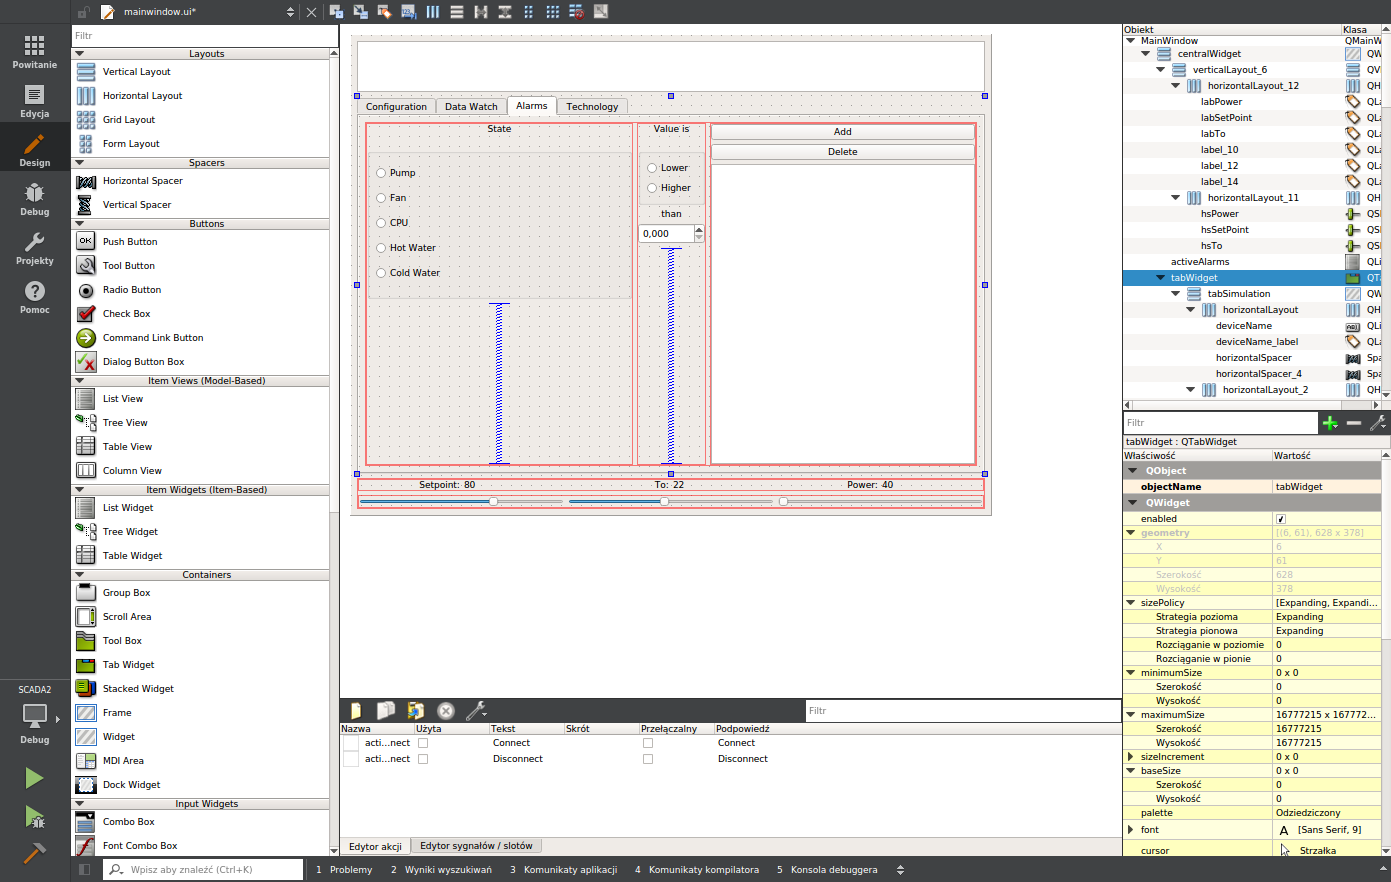
\includegraphics[width=\textwidth]{../img/qtcreator.png}
    \caption{Widok okna \textit{Design} programu \textit{Qt Creator}}
    \label{fig:qtcreator}
\end{figure}

Pierwszym skojarzeniem w~tym miejscu jest okno służące do tworzenia paneli
operatorskich w~programie \textit{zenon}. Chociaż mają one zupełnie różne
zastosowania, to w~podobny sposób pozwalają na rozmieszczanie elementów zgodnie
z~zasadą WYSIWYG (ang. What You See Is What You Get).

\subsection{Okno programu}
\indent

\begin{figure}[!ht]
    \centering
    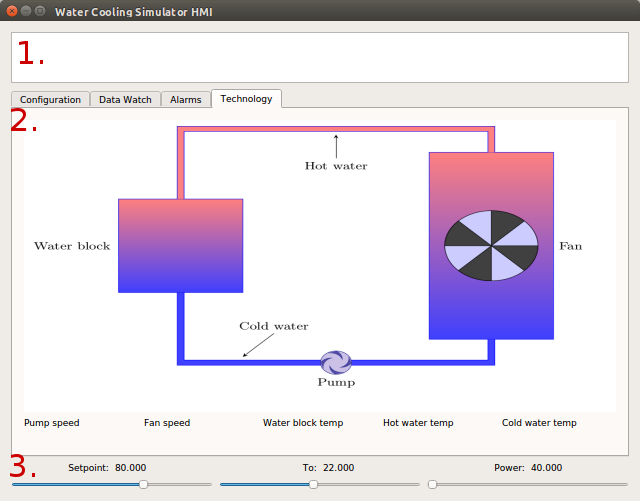
\includegraphics[width=0.75\textwidth]{../img/mainwindow.png}
    \caption{Okno programu}
    \label{fig:mainwindow}
\end{figure}

Na rysunku~\ref{fig:mainwindow} przedstawione zostało okno stworzonego programu.
Zawiera ono trzy główne części oznaczone numerami na powyższym rysunku:
\begin{enumerate}
    \item Okno aktywnych alarmów.
    \item Zakładki z~oknami:
        \begin{itemize}
            \item  konfiguracji połączenia oraz parametrów regulatorów,
            \item prezentacji danych w~formie wykresu w~funkcji czasu,
            \item konfiguracji alarmów,
            \item panelu technologii.
        \end{itemize}
    \item Suwaki nastaw parametrów symulacji.
\end{enumerate}

\newpage
\subsection{Panel technologii}
\indent

\begin{figure}[!ht]
    \centering
    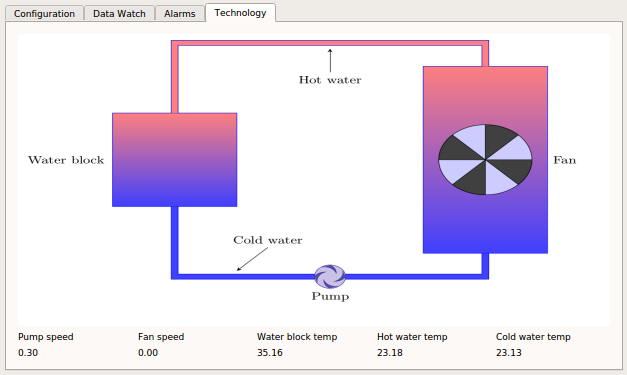
\includegraphics[width=\textwidth]{../img/technology.png}
    \caption{Panel technologii}
    \label{fig:technology}
\end{figure}

Panel technologii został przedstawiony na rysunku~\ref{fig:technology}. Jego
główną częścią jest schemat technologiczny procesu, pod którym znajdują się pola
wyświetlające wartości zmiennych stanu odpowiadających odpowiednim elementom
tego schematu.

W~trakcie pracy, po podłączeniu do płytki, w~czasie rzeczywistym wyświetlane są
tam wszystkie zmienne, co przypomina ekrany technologii tworzone w~programie
\textit{zenon}. W~przeciwieństwie jednak do specjalistycznego oprogramowania,
widoczny na rysunku~\ref{fig:technology} ekran nie pozwala na animowanie
odpowiednich elementów składowych procesu zgodnie z~aktualnym stanem systemu,
gdyż jest on jedynie grafiką. W~tym przypadku znacznie wygodniejszym do tego
narzędziem jest program typu SCADA, który z~założenia pozwala na interaktywną
reprezentację procesu, jednak należy nadmienić, iż nic nie stoi na przeszkodzie,
aby z~wykorzystaniem narzędzi dostarczanych przez bibliotekę \textit{Qt} w~razie
potrzeby przygotować odpowiednie funkcjonalności.

\newpage
\subsection{Panel prezentacji danych --~\textit{Data Watch}}
\indent

\begin{figure}[!ht]
    \centering
    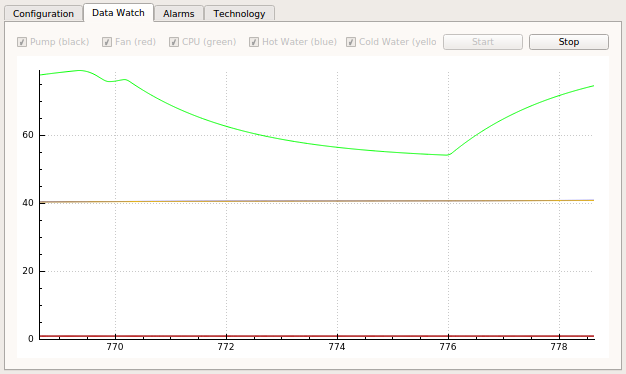
\includegraphics[width=\textwidth]{../img/datawatch.png}
    \caption{Panel prezentacji danych}
    \label{fig:datawatch}
\end{figure}

Panel prezentacji danych na wykresie w~funkcji czasu przedstawiony został na
rysunku~\ref{fig:datawatch}. Składa się on z~dwóch głównych elementów:
\begin{itemize}
    \item wyboru danych do prezentacji,
    \item wykresu wartości zmiennych stanu w~funkcji czasu.
\end{itemize}

Konfiguracja polega na zaznaczeniu zmiennych, które mają znaleźć się na wykresie
oraz naciśnięciu przycisku \textit{Start}, który powoduje rozpoczęcie rysowania
przebiegu wartości zmiennych stanu w~funkcji czasu. W~trakcie tego procesu
niemożliwa jest zmiana liczby wyświetlanych zmiennych. W~tym celu należy
zatrzymać rysowanie przyciskiem \textit{Stop}, a~następnie dobrać nową
konfigurację.

Wykres tworzony jest z~wykorzystaniem biblioteki \textit{QCustomPlot}, która
pozwala na dowolną konfigurację sposobu prezentacji danych. Otrzymane przebiegi
odpowiadają tym, które możliwe są do uzyskania przy pomocy trendów w~programie
\textit{zenon} lub bezpośrednio poprzez oprogramowanie producentów sterowników
\textit{PLC}. Oczywistym jest, że stworzenie kodu pozwalającego na przyjazne
użytkownikowi konfigurowanie ilości prezentowanych danych jest nieco bardziej
pracochłonnym procesem, aniżeli umieszczenie odpowiednich elementów w~panelu
operatorskim specjalistycznego oprogramowania typu SCADA, jednak biblioteka
\textit{QCustomPlot} zawiera bardzo przejrzysty interfejs, który umożliwia
relatywnie szybkie jej użycie. Dzięki temu udało się uzyskać efekt działania
zbliżony do tego znanego chociażby z~programu \textit{zenon}.

\newpage
\subsection{Panel konfiguracji alarmów}
\indent

\begin{figure}[!ht]
    \centering
    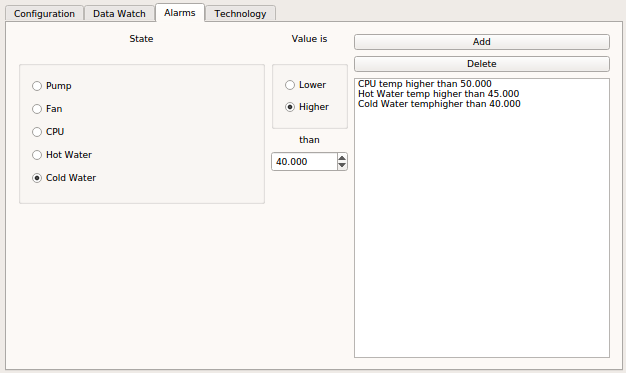
\includegraphics[width=\textwidth]{../img/confalarms.png}
    \caption{Panel konfiguracji alarmów}
    \label{fig:confalarms}
\end{figure}

Panel konfiguracji alarmów przedstawiony został na rysunku~\ref{fig:confalarms}.
Pozwala on na:
\begin{itemize}
    \item wybór zmiennej stanu,
    \item wybór rodzaju alarmu --~przekroczenie górnego lub dolnego progu,
    \item wybór poziomu granicznego uaktywniającego alarm.
\end{itemize}

Ustawienie alarmu polega na wybraniu zmiennej stanu, następnie określany jest
rodzaj tego alarmu --~czy ma się on uaktywnić po uzyskaniu przez zmienną stanu
wartości wyższej, czy też niższej od zadanej --~oraz progu, którego
przekroczenie powoduje, iż alarm zostaje uaktywniony. Na
rysunku~\ref{fig:confalarms} przedstawiona jest sytuacja, w~której ustawione
zostały trzy aktywne alarmy informujące o~uzyskaniu temperatur wyższych od
zadanych dla procesora, wody ciepłej oraz wody zimnej.

Rysunek~\ref{fig:activealarms} przedstawia sytuację, w~której dodatkowo zostały
ustawione alarmy dla poziomów pracy pompy wody oraz wentylatorów i~zasymulowana
została sytuacja dostarczenia do systemu maksymalnej mocy cieplnej. W~wyniku
tego działania przekroczeniu uległy zadane wartości progowe dla ustawionych
alarmów i~pojawiły się one w~oknie alarmów aktywnych.

\newpage
\begin{figure}[!ht]
    \centering
    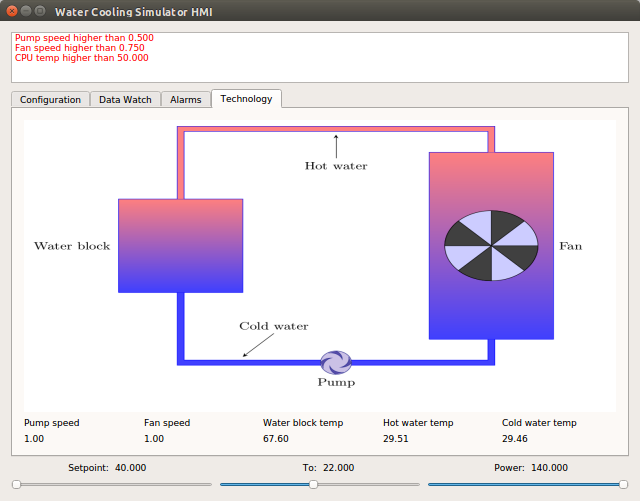
\includegraphics[width=\textwidth]{../img/activealarms.png}
    \caption{Okno programu z~aktywnymi alarmami}
    \label{fig:activealarms}
\end{figure}

Działanie panelu konfiguracji alarmów jest bardzo zbliżone do tego znanego
z~programu \textit{zenon}, przy czym, zdaniem autorów, dzięki pisaniu kodu po
zaznajomieniu z~funkcjonalnością specjalistycznego oprogramowania udało się
uzyskać interfejs bardziej przejrzysty i~łatwiejszy w~zarządzaniu, a~dodatkowo
niewiele ustępujący podstawowym możliwościom znanym z~profesjonalnego środowiska
typu SCADA.

\newpage
\subsection{Panel konfiguracji połączenia i~regulatorów}
\indent

\begin{figure}[!ht]
    \centering
    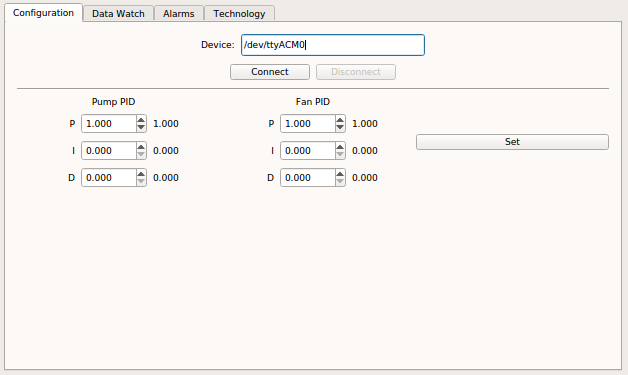
\includegraphics[width=\textwidth]{../img/config.png}
    \caption{Panel konfiguracji połączenia i~regulatorów}
    \label{fig:config}
\end{figure}

Panel służący do konfiguracji połączenia i~parametrów regulatorów przedstawiony
został na rysunku~\ref{fig:config}. Jego podstawowym elementem jest miejsce do
wprowadzenia nazwy portu szeregowego, który służy do komunikacji z~płytką, na
której symulowane jest działanie układu chłodzenia cieczą. Sama komunikacja po
stronie komputera została wykonana z~wykorzystaniem interfejsu \textit{POSIX},
gdyż oprogramowanie tworzone było na system \textit{Linux}. Istnieje również
możliwość komunikacji pod systemem z~rodziny \textit{Windows}, jednak
w~tworzonym projekcie funkcjonalność taka nie została zaimplementowana z~powodu
braku środowiska testowego.

Dodatkowo panel ten zawiera elementy służące do wyboru nastaw regulatorów, które
po ustawieniu i~zatwierdzeniu przyciskiem \textit{Set} są przesyłane do programu
uruchomionego na płytce. Funkcjonalność ta została dodana niejako dodatkowo, aby
ułatwić testowanie stworzonego oprogramowania.

\newpage
\subsection{Suwaki nastaw parametrów symulacji}
\indent

\begin{figure}[!ht]
    \centering
    
\includegraphics[width=\textwidth]{../img/sliders.png}
    \caption{Suwaki nastaw parametrów symulacji}
    \label{fig:sliders}
\end{figure}

Rysunek~\ref{fig:sliders} przedstawia suwaki nastaw parametrów symulacji, które
znajdują się w~dolnej części okna programu. Ich wartości są na bieżąco
przesyłane do programu uruchomionego na płytce, dzięki czemu możliwe jest
odtworzenie różnych zachowań systemu. Pozwalają one na następujące nastawy:
\begin{itemize}
    \item wybór wartości zadanej (temperatury procesora) z~zakresu od $40$ do
    $100$~[$^\circ C$],
    \item wybór temperatury otoczenia radiatora z~zakresu od $15$ do
    $30$~[$^\circ C$],
    \item wybór mocy cieplnej dostarczanej do systemu z~zakresu od $40$ do
    $140$~[$W$].
\end{itemize}

Przykładowe wykorzystanie powyższych suwaków widoczne było w~przypadku opisu
okna prezentacji danych, gdzie odpowiednie przebiegi
z~rysunku~\ref{fig:datawatch} zostały uzyskane poprzez manipulowanie mocą
cieplną dostarczaną do systemu. Również rysunek~\ref{fig:activealarms}
przedstawiający aktywne alarmy został uzyskany w~podobny sposób, gdyż
zwiększenie dostarczanej mocy oraz obniżenie wartości zadanej pozwoliły na
uaktywnienie odpowiednich alarmów.
